\documentclass[12pt, twoside]{article}
\usepackage[letterpaper, margin=0.25in, head=30pt, headsep=0.1in]{geometry}
\usepackage[english]{babel}
\usepackage[utf8]{inputenc}
\usepackage{amsmath}
\usepackage{amsfonts}
\usepackage{amssymb}
\usepackage{tikz}
\usetikzlibrary{quotes, angles}

\usepackage{graphicx}
\usepackage{enumitem}
\usepackage{multicol}

%\usepackage{pgfplots}
%\pgfplotsset{width=10cm,compat=1.9}
%\usepgfplotslibrary{statistics}
%\usepackage{pgfplotstable}
%\usepackage{tkz-fct}
%\usepackage{venndiagram}

\usepackage{fancyhdr}
\pagestyle{fancy}
\fancyhf{}
\renewcommand{\headrulewidth}{0pt} % disable the underline of the header
\raggedbottom
\newif\ifmeta
\metatrue %print standards and topics tags

\title{Math AI Worksheet Generator and Formative Assessment System}
\author{Chris Huson}
\date{November 2020}

%\fancyhead[RE]{\thepage}
%\fancyhead[RO]{\thepage \\ Name: \hspace{3cm}}
%\fancyhead[L]{BECA / Dr. Huson / 10th Grade Geometry\\* 7 June 2019}
%
%\begin{document}
%\subsubsection*{13.7 Homework: Cross sections, distance applications}
%\fancyhead[L]{BECA / Dr. Huson / Geometry 03-Volume+angle-bisectors\\* pset ID: 34}

\begin{document}

\subsubsection*{3.3 Volume of a prism}
\begin{enumerate}
  \item Do Now: As shown below, two lines intersect making four angles: $\angle 1$, $\angle 2$, $\angle 3$, and $\angle 4$.
  \begin{center}
  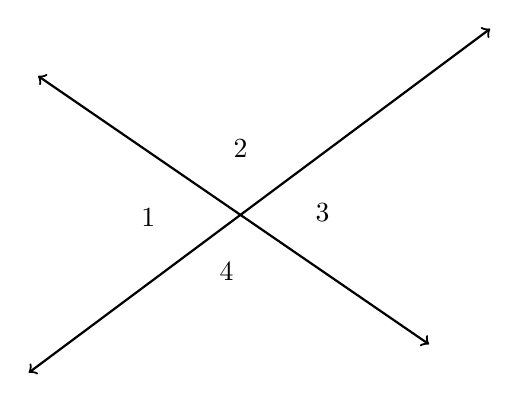
\begin{tikzpicture}[scale=0.7, rotate=20]
    \draw [<->, thick] (0,-1.5)--(10,1.5);
    \draw [<->, thick] (2,3.5)--(7,-3.5);
    \node at (3,.4){1};
    \node at (6,-.6){3};
    \node at (5,1){2};
    \node at (4,-1){4};
    %\draw [fill] (0,0) circle [radius=0.05] node[below]{$P$};
    %\draw [fill] (6,0) circle [radius=0.05] node[below]{$R$};
    %\draw [fill] (3,0) circle [radius=0.05] node[below]{$Q$};
  \end{tikzpicture}
  \end{center}
  \begin{enumerate}
  \item Which angle is opposite $\angle 1$? \rule{4cm}{0.15mm} \bigskip
  \item Name an angle that is adjacent to $\angle 4$. \rule{4cm}{0.15mm} \bigskip
  \item True or false, $\angle 2$ and $\angle 4$ are vertical angles. \rule{3cm}{0.15mm}
\end{enumerate}
  
\newpage
\item Do Now: The horizontal line segment $\overline{RS}$ is plotted on the coordinate plane with $R(2,3)$ and $S(7,3)$. 
  \begin{multicols}{2}
    Find length $RS$, showing the calculation.
      \begin{flushright}
      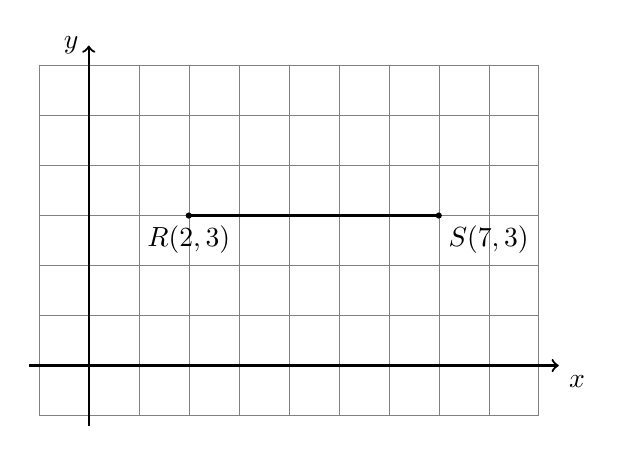
\begin{tikzpicture}[scale=.635]
        \draw [help lines] (-1,-1) grid (9,6);
        \draw [thick, ->] (-1.2,0) -- (9.4,0) node [below right] {$x$};
        \draw [thick, ->] (0,-1.2)--(0,6.4) node [left] {$y$};
        \draw [-, thick] (2,3)--(7,3);
        \draw [fill] (2,3) circle [radius=0.05] node[below]{$R(2,3)$};
        \draw [fill] (7,3) circle [radius=0.05] node[below right]{$S(7,3)$};
      \end{tikzpicture}
      \end{flushright}
  \end{multicols} 

\newpage
\item Do Now: The vertical line segment $\overline{PQ}$ is plotted on the coordinate plane with $P(3,5)$ and $Q(3,1)$. 
  \begin{multicols}{2}
    Find the length $PQ$. \\[0.5cm]
    Show the calculation, including the absolute value bars.
      \begin{flushright}
      \begin{tikzpicture}[scale=.635]
        %\draw [help lines] (-1,-1) grid (9,9);
        \draw [thick, ->] (-1.2,0) -- (9.4,0) node [below right] {$x$};
        \draw [thick, ->] (0,-1.2)--(0,7.4) node [left] {$y$};
        \draw [-, thick] (3,5)--(3,1);
        \draw [fill] (3,5) circle [radius=0.05] node[right]{$P(3,5)$};
        \draw [fill] (3,1) circle [radius=0.05] node[right]{$Q(3,1)$};
      \end{tikzpicture}
      \end{flushright}
  \end{multicols} 


\newpage
\item Take notes: The volume of a box (rectanglar prism) is the product of its length, width, and height.
$$V = l \times w \times h$$
Example: Find the volume of a box with a length of 8 centimeters, a depth of 4 cm, and a height of 5 cm. Show the calculation.
\begin{flushright}
  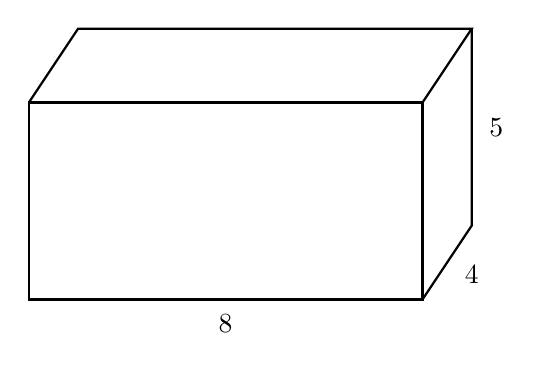
\begin{tikzpicture}[scale=1.25]
    \draw [-, thick] (0,0)--(4,0)--(4,2)--(0,2)--cycle;
    \draw [-, thick] (0,2)--(0.5,2.75)--(4.5,2.75)--(4,2);
    \draw [-, thick] (4,0)--(4.5,0.75)--(4.5,2.75);
    \node at (4.75, 1.75){$5$};
    \node at (2, -0.25){$8$};
    \node at (4.5, 0.25){$4$};
  \end{tikzpicture}
  \end{flushright} \vspace{2cm} 

\newpage
\item Find the volume of a box (rectanglar prism) having a length of 12 inches, a width of 6 inches, and a height of 5 inches. Show the calculation.

\newpage
\begin{multicols*}{2}
\item Given $\overline{ABC}$, $AB=84$, $AC=116$.\\ [0.25cm]
  Find ${BC}$.\\[1.5cm]
      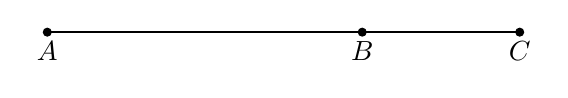
\begin{tikzpicture}
        \draw [-, thick] (1,0)--(7,0);
        \draw [fill] (1,0) circle [radius=0.05] node[below]{$A$};
        \draw [fill] (5,0) circle [radius=0.05] node[below]{$B$};
        \draw [fill] (7,0) circle [radius=0.05] node[below]{$C$};
      \end{tikzpicture} \vspace{2cm}
\columnbreak

\item Given $\overline{DEF}$, $DE=3 \frac{1}{3}$, and $EF=4 \frac{1}{6}$. \\ [0.25cm]
  Find ${DF}$.\\[1.5cm]
      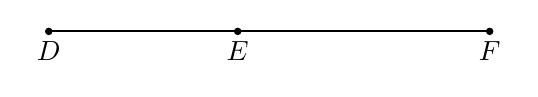
\begin{tikzpicture}[scale=0.8]
        \draw [-, thick] (0,0)--(7,0);
        \draw [fill] (0,0) circle [radius=0.05] node[below]{$D$};
        \draw [fill] (3,0) circle [radius=0.05] node[below]{$E$};
        \draw [fill] (7,0) circle [radius=0.05] node[below]{$F$};
      \end{tikzpicture} \vspace{2cm}
    \end{multicols*}

\newpage
\item Answer based on the diagram below. \vspace{0.25cm}
  \begin{enumerate}
    \item Name an angle that is supplementary to $\angle AOB$: \rule{4cm}{0.15mm} \bigskip
    \item Name an angle that is complementary to $\angle DOE$: \rule{4cm}{0.15mm}
  \end{enumerate}
  \begin{center}
  \begin{tikzpicture}[scale=1.0, rotate=-20]
    \draw [<->, thick] (-55:3)--(0,0)--(125:4);
    \draw [<->, thick] (-5,0)--(5,0);
    \draw [->, thick] (0,0)--(0,4);
    \draw (0,0)++(0.3,0)--++(0,0.3)--+(-0.3,0);
    %\draw [fill] (-1,2.5) circle [radius=0.05] node[left ]{$B$};
    \draw [fill] (125:3) circle [radius=0.05] node[below left]{$B$};
    \draw [fill] (-4,0) circle [radius=0.05] node[below]{$A$}; 
    \draw [fill] (0,0) circle [radius=0.05] node[below left]{$O$};
    \draw [fill] (0,3) circle [radius=0.05] node[left]{$C$};
    \draw [fill] (4,0) circle [radius=0.05] node[below]{$D$};
    \draw [fill] (-55:2) circle [radius=0.05] node[left]{$E$};
  \end{tikzpicture}
  \end{center}

\newpage
\item Given $\overleftrightarrow{PQ}$ as shown on the number line. Find $PQ$. \\[20pt] % Midpoint
      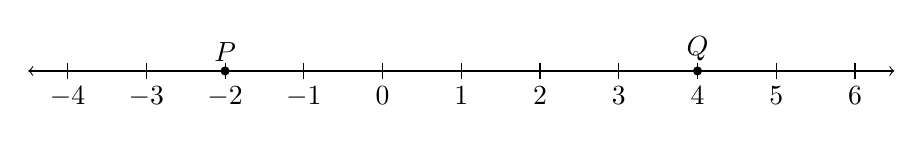
\begin{tikzpicture}
        \draw [<->] (-4.5,0)--(6.5,0);
        \foreach \x in {-4,...,6} %2 leading for diff!=1
          \draw[shift={(\x,0)},color=black] (0pt,-3pt) -- (0pt,3pt) node[below=5pt]  {$\x$};
          \draw [fill] (-2,0) circle [radius=0.05] node[above] {$P$};
          \draw [fill] (4,0) circle [radius=0.05] node[above] {$Q$};
      \end{tikzpicture} \\ \bigskip
      \vspace{1cm}  
  
  \item Given $\overleftrightarrow{RS}$, with $R=0.7$ and $S=5.3$. Find $RS$, showing the formula.\\[20pt]
      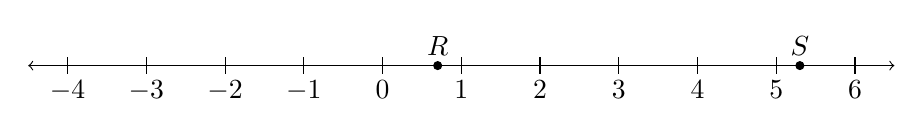
\begin{tikzpicture}
        \draw [<->] (-4.5,0)--(6.5,0);
        \foreach \x in {-4,...,6} %2 leading for diff!=1
          \draw[shift={(\x,0)},color=black] (0pt,-3pt) -- (0pt,3pt) node[below=5pt]  {$\x$};
          \draw [fill] (0.7,0) circle [radius=0.05] node[above] {$R$};
          \draw [fill] (5.3,0) circle [radius=0.05] node[above] {$S$};
      \end{tikzpicture} \\ \bigskip

  
\newpage
\item Given the situation in the diagram, answer each question. Circle True or False. 
  \vspace{0.25cm}
      \begin{center}
      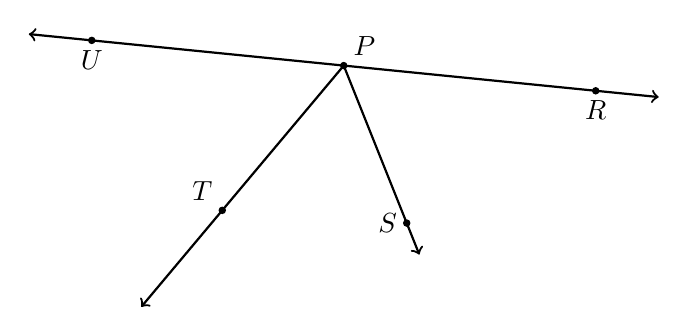
\begin{tikzpicture}[scale=0.8, rotate=180]
        \draw [->, thick] (0,0)--(50:5);
        \draw [<->, thick] (-5,.5)--(5,-.5);
        \draw [->, thick] (0,0)--(-1.2,3);
        \draw [fill] (-1,2.5) circle [radius=0.05] node[left ]{$S$};
        \draw [fill] (50:3) circle [radius=0.05] node[above left ]{$T$};
        \draw [fill] (0,0) circle [radius=0.05] node[above right]{$P$};
        \draw [fill] (4,-0.4) circle [radius=0.05] node[below]{$U$};
        \draw [fill] (-4,0.4) circle [radius=0.05] node[below]{$R$};
      \end{tikzpicture}
      \end{center}
    \begin{enumerate}
      \item True or False: $\overrightarrow{RP}$ and $\overrightarrow{UP}$ are opposite rays.\bigskip
      \item True or False: $\angle TPR$ is supplementary to $\angle TPU$.\bigskip
      \item True or False: $\angle RPS$ and $\angle TPS$ are complementary angles. \bigskip
      \item True or False: $\angle RPS$ and $\angle TPU$ are vertical angles. \bigskip
    \end{enumerate}

\newpage
\item The shape shown below is composed of straight lines and right angles, with some lengths as marked. Find the perimeter of the figure. Show your work.
    \begin{flushright}
    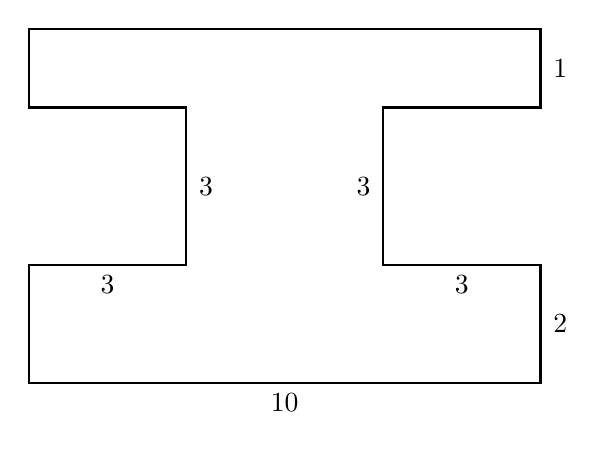
\begin{tikzpicture}[scale=0.5]
      \draw [-, thick] (0,0)--(13,0)--(13,3)--(9,3)--(9,7)--(13,7)--
      (13, 9)--(0,9)--(0,7)--(4,7)--(4,3)--(0,3)--cycle;
      %\draw [fill] (0,0) circle [radius=0.05] node[left]{$A$};
      %\draw [fill] (7,0) circle [radius=0.05] node[right]{$B$};
      %\draw [fill] (7,2) circle [radius=0.05] node[right]{$C$};
      %\draw [fill] (0,2) circle [radius=0.05] node[left]{$D$};
      \node at (4.5, 5){3};
      \node at (2, 2.5){3};
      \node at (8.5, 5){3};
      \node at (11, 2.5){3};
      \node at (6.5, -0.5){10};
      \node at (13.5, 1.5){2};
      \node at (13.5, 8){1};
    \end{tikzpicture}
    \end{flushright} 

\newpage
\item Given $\overline{DEFG}$, $DE=1 \frac{2}{5}$, $EF=2 \frac{3}{10}$, and $FG= \frac{4}{5}$. (diagram not to scale)\\ [0.25cm]
  Find ${DG}$, expressed as a fraction, not a decimal.
  \begin{flushright}
      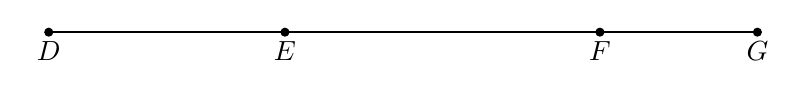
\begin{tikzpicture}
        \draw [-, thick] (0,0)--(9,0);
        \draw [fill] (0,0) circle [radius=0.05] node[below]{$D$};
        \draw [fill] (3,0) circle [radius=0.05] node[below]{$E$};
        \draw [fill] (7,0) circle [radius=0.05] node[below]{$F$};
        \draw [fill] (9,0) circle [radius=0.05] node[below]{$G$};
      \end{tikzpicture}
    \end{flushright}

\newpage
\item Given the rectangle $ABCD$ shown below, with $AB=6 \frac{1}{3}$ and $BC=2 \frac{1}{2}$. Find the area of the rectangle, expressing your result as a fraction.
\begin{flushright}
\begin{tikzpicture}[scale=1.25]
  \draw [-, thick] (0,0)--(4.5,0)--(4.5,2)--(0,2)--cycle;
  \draw [fill] (0,0) circle [radius=0.05] node[left]{$A$};
  \draw [fill] (4.5,0) circle [radius=0.05] node[right]{$B$};
  \draw [fill] (4.5,2) circle [radius=0.05] node[right]{$C$};
  \draw [fill] (0,2) circle [radius=0.05] node[left]{$D$};
  \node at (5, 1){$2 \frac{1}{2}$};
  \node at (2.25, -0.5){$6 \frac{1}{3}$};
\end{tikzpicture}
\end{flushright} \vspace{2cm}  

\end{enumerate}
\end{document}